\chapter{Methods and Results}
\label{chapter:methods}

In figure \ref{fig:image}, the processing pipeline for this project is shown.

\begin{figure}[h!]
    \centering
    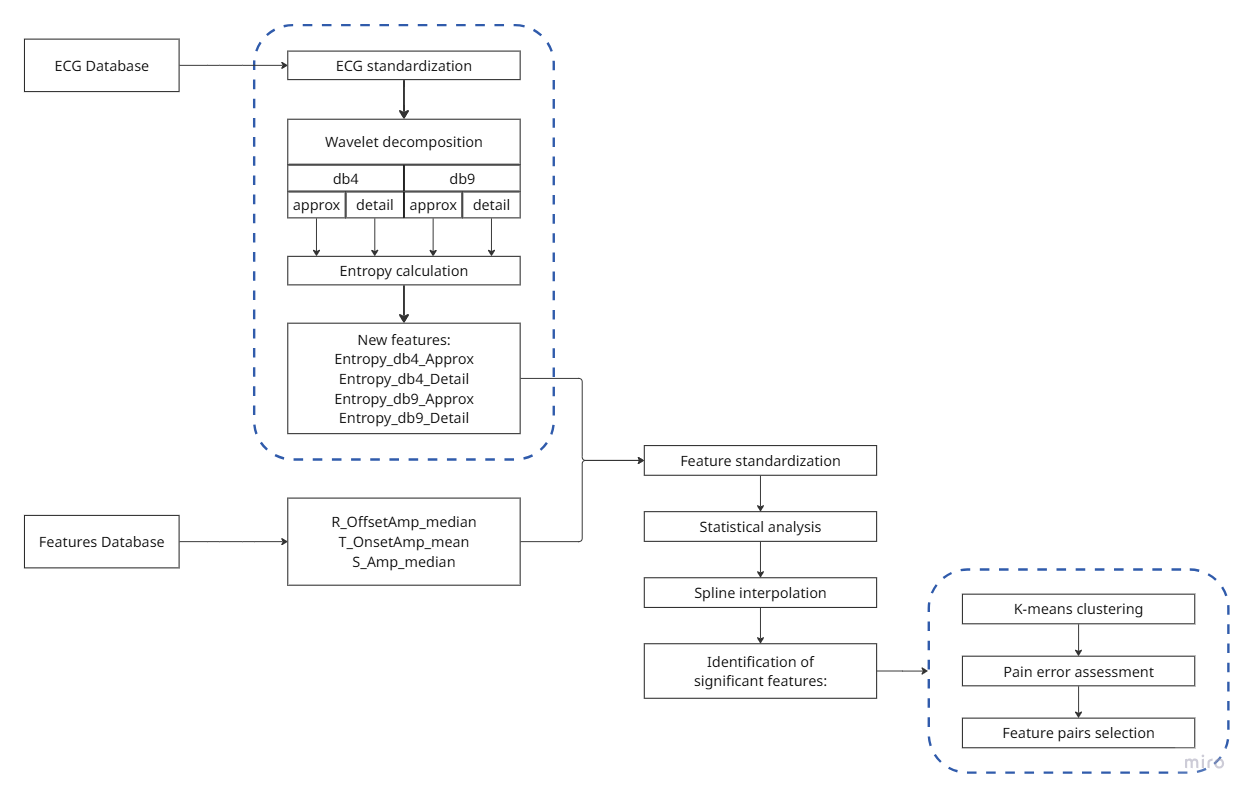
\includegraphics[width=1.0\textwidth]{image.png}
    \caption{Processing pipeline.}
    \label{fig:image}
\end{figure}

\section{Database Acquisition}
In this project, two databases were used: one has data from an \ac{ecg} signal while the other contains features extracted from that \ac{ecg}, as described in the article by Bruna et al \cite{Alves2024}.

The protocol that was carried out to create the databases began with a 5-minute baseline period, during which only physiological signals were collected while participants sat in a relaxed position without any stimuli. 
Next, participants viewed a 10-minute video composed of segments from comedy, horror or documentary films to elicit positive, negative or neutral emotional states, respectively. 
After the video, another 5-minute stimuli-free period was conducted. 
Following this, participants immersed their non-dominant hand in a tank of cold water (7 ± 1°C), inducing pain through a Cold Pressor Test(\ac{cpt}), and reported their pain using the \ac{nps} at four key points: before immersing their hand, when pain was first felt (Pain Threshold), when the pain became unbearable (Pain Tolerance) and 3 minutes after removing their hand from the water. 
The CPT section ended when the limit of pain tolerance was reached, or after 2 minutes if the participant didn’t reach theirs before that. 
Finally, the 5-minute period with no stimuli was repeated, being characterized as a rest period. This process is depicted in figure. 

During the study, three physiological signals were recorded, more precisely, ECG, EDA and EMG from trapezius and triceps muscles. The ECG was recorded in a database, that was later used in this project.
Following up in the article, heart rate (HR), the amplitude of wave peaks, the amplitude of onsets and offsets of the waves (???), the distance between consecutive onsets and offsets and the distance between consecutive peaks were extracted in the form of time series, using 10-second windows with 50\% overlap. 
Then, for all of these, statistical metrics, like the mean, median and variance, were computed for each window, resulting in 237 features that were later processed. These are all included in the features database, also used in this project.



\section{Feature Extraction}
In the aforementioned article, the features of the ECG that can be used to best describe pain are defined.
Hence, the top four features were selected for analysis, namely, the median of the R wave offset amplitude, the median of the T wave onset amplitude, and the mean and median of the S wave peak amplitude.



\section{Data Analysis}
To do the optimal processing of the features, five participants were selected at random, while ensuring the videos watched by them were different. 
Once this was done, graphics of the features in function of time were plotted for each participant. 
An example can be seen in figure 3, in which a clear change can be seen when the participant dips their hand in water, feeling pain. 









